%\documentstyle[epsf,twocolumn]{jarticle}       %LaTeX2.09仕様
\documentclass[twocolumn]{jarticle}     %pLaTeX2e仕様

%\usepackage[backend=bibtex, style=numeric]{biblatex}
%\addbibresource{sankou.bib}
%%%%%%%%%%%%%%%%%%%%%%%%%%%%%%%%%%%%%%%%%%%%%%%%%%%%%%%%%%%%%%
%%
%%  基本 バージョン
%%
%%%%%%%%%%%%%%%%%%%%%%%%%%%%%%%%%%%%%%%%%%%%%%%%%%%%%%%%%%%%%%%%
\setlength{\topmargin}{-45pt}
%\setlength{\oddsidemargin}{0cm}
\setlength{\oddsidemargin}{-7.5mm}
%\setlength{\evensidemargin}{0cm}
\setlength{\textheight}{24.1cm}
%setlength{\textheight}{25cm}
\setlength{\textwidth}{17.4cm}
%\setlength{\textwidth}{172mm}
\setlength{\columnsep}{11mm}

\setlength{\intextsep}{8pt}
\setlength{\textfloatsep}{8pt}
\setlength{\floatsep}{1pt}

\kanjiskip=.07zw plus.5pt minus.5pt



%【節がかわるごとに(1.1)(1.2) …(2.1)(2.2)と数式番号をつけるとき】
%\makeatletter
%\renewcommand{\theequation}{%
%\thesection.\arabic{equation}} %\@addtoreset{equation}{section}
%\makeatother

%\renewcommand{\arraystretch}{0.95} 行間の設定

\usepackage[dvipdfmx]{graphicx}   %pLaTeX2e仕様(\documentstyle ->\documentclass)
\usepackage{scalefnt}
\usepackage{bm}
\usepackage{url}
\usepackage{amsmath}
\usepackage{amsfonts}
\usepackage[subrefformat=parens]{subcaption}
\captionsetup{compatibility=false}
%%%%%%%%%%%%%%%%%%%%%%%%%%%%%%%%%%%%%%%%%%%%%%%%%%%%%%%%
\usepackage{comment}
\usepackage{subcaption}
\usepackage{multirow}
\usepackage{nidanfloat}
\usepackage[dvipdfmx]{hyperref}

\usepackage[normalem]{ulem}
\useunder{\uline}{\ul}{}

\begin{document}

\twocolumn[
\noindent
\hspace{1em}

令和2年4月29日(水) ゼミ資料
\hfill
\ \ B4 高山 裕成

\vspace{2mm}
\hrule
\begin{center}
{\Large  進捗報告}
\end{center}
\hrule
\vspace{3mm}
]

\section{あらすじ}
B3 実験において, 「自然言語処理と深層学習に基づいた 4 コマ漫画のセリフの感情推定」を行った.

そして, 今学期において最初のタスクとしては BERT\cite{BERT} による分散表現を獲得し, B3 実験と同様に感情推定を行い, 結果の比較・考察をすることであった.
先週からのタスクとしては BERT の fine-tuning が挙げられる.

% \footnotesize
\section{今週やったこと}

\begin{itemize}
  \item BERT の fine-tuning 実装.
  \item ``1g-hub/bert\_practice" レポジトリ作成.
\end{itemize}

\section{BERT の fine-tuning 実装}
optuna を用いて最適パラメータを出した後, 最適パラメータを用いて fine-tuning 出来るようになった. 以下の問題設定で, fine-tuning が動作することを確かめた. 実行ソースコードは ``1g-hub/takayama/src/ex\_2020\_4\_29.py" にある.

\begin{itemize}
  \item 入力は 1 つのセリフ文の単語 id 列, 出力は感情ラベル(0:'喜楽', 1:'その他')
  \item クラス重みは正規化されたラベル逆比
  \item BERT の事前学習済モデルは日本語 Wikipedia から 全 1,800 万文を用いて事前学習させたモデル\footnote{http://nlp.ist.i.kyoto-u.ac.jp}を利用した.
  \item BERT の出力に 全結合層 (Classification layer) をアダプトし, 両方のパラメータを学習.
  \item optuna でチューニングするのは時短のため learning rate のみ. 試行回数は 5 回.
  \item B3 実験で用いていた learning rate scheduler は不使用.
\end{itemize}

学習パラメータを表\ref{table:ex_para}, ネットワークの概略図を図\ref{fig:net} に示す.

\begin{table}
\caption{学習パラメータ}
\label{table:ex_para}
\centering
\begin{tabular}{|c||c|c|}
\hline
& \multicolumn{2}{|c|}{実験 $1・2$} \\ \hline
epoch & \multicolumn{2}{|c|}{20}  \\ \hline
batch size & \multicolumn{2}{|c|}{32} \\ \hline
loss function & \multicolumn{2}{|c|}{Cross Entropy Loss} \\ \hline
optimizer & \multicolumn{2}{|c|}{Adam} \\ \hline
\end{tabular}
\end{table}


\begin{figure}[htb]
  \begin{center} %センタリングする
    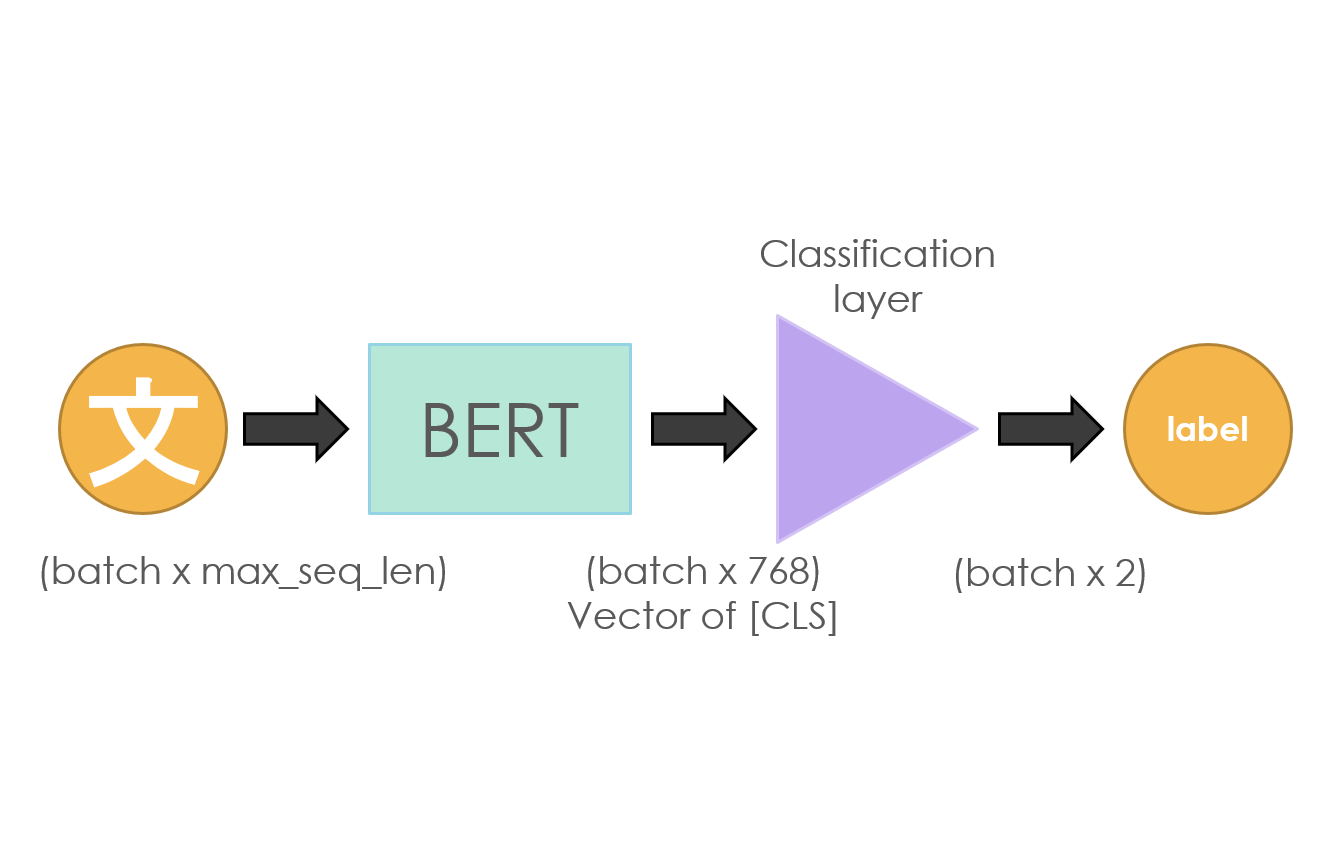
\includegraphics[width=7.0cm]{net.png}
    \caption{model} %タイトルをつける
    \label{fig:net} %ラベルをつけ図の参照を可能にする
  \end{center}
\end{figure}

\section{BERT fine-tuning テスト動作 結果}
テスト動作の結果を表\ref{tab:result} に示す.
$D2V + MLP$, $D2V + SVM$, $D2V + RF$ は B3 実験にて得た, 同様の問題設定で分散表現化手法として Doc2Vec を用い, 識別器として, 3 層からなる多層パーセプトロン (MLP), SVM, RandomForest (RF) を用いた感情推定の結果である. (epoch 数や batch size は異なる.)

計算時間は約 15 sec / epoch であった. あまり良い結果ではなかったが, これがバグによるものなのか, 時短方策によるものなのかは定かではない. 図\ref{fig:gyagu} にギャグタッチにおける, loss, accuracy, 正例の F1 値の遷移を示している. 図\ref{fig:gyagu} を見る限りはうまく学習出来ていない.

\begin{table}[h]
\begin{center}
\caption{result}
\begin{tabular}{c|ccc}
\hline
\multirow{2}{*}{識別器} & \multicolumn{3}{c|}{5 タッチ平均} \\ \cline{2-4}
 & Acc & \multicolumn{1}{c}{Recall} & \multicolumn{1}{c}{F1} \\ \hline
D2V + MLP & \multicolumn{1}{l}{0.66} & 0.32 & 0.31 \\
D2V + SVM & \multicolumn{1}{l}{0.65} & 0.19 & 0.19 \\
D2V + RF & \multicolumn{1}{l}{0.67} & 0.19 & 0.20 \\
BERT fine-tuning & 0.70 & \multicolumn{1}{c}{0.30} & \multicolumn{1}{c}{0.21} \\ \hline
ベースライン & 0.71 & \multicolumn{1}{c}{0.00} & \multicolumn{1}{c}{0.00} \\ \hline
\end{tabular}
\label{tab:result}
\end{center}
\end{table}

\begin{figure}[h]
  \begin{center} %センタリングする
    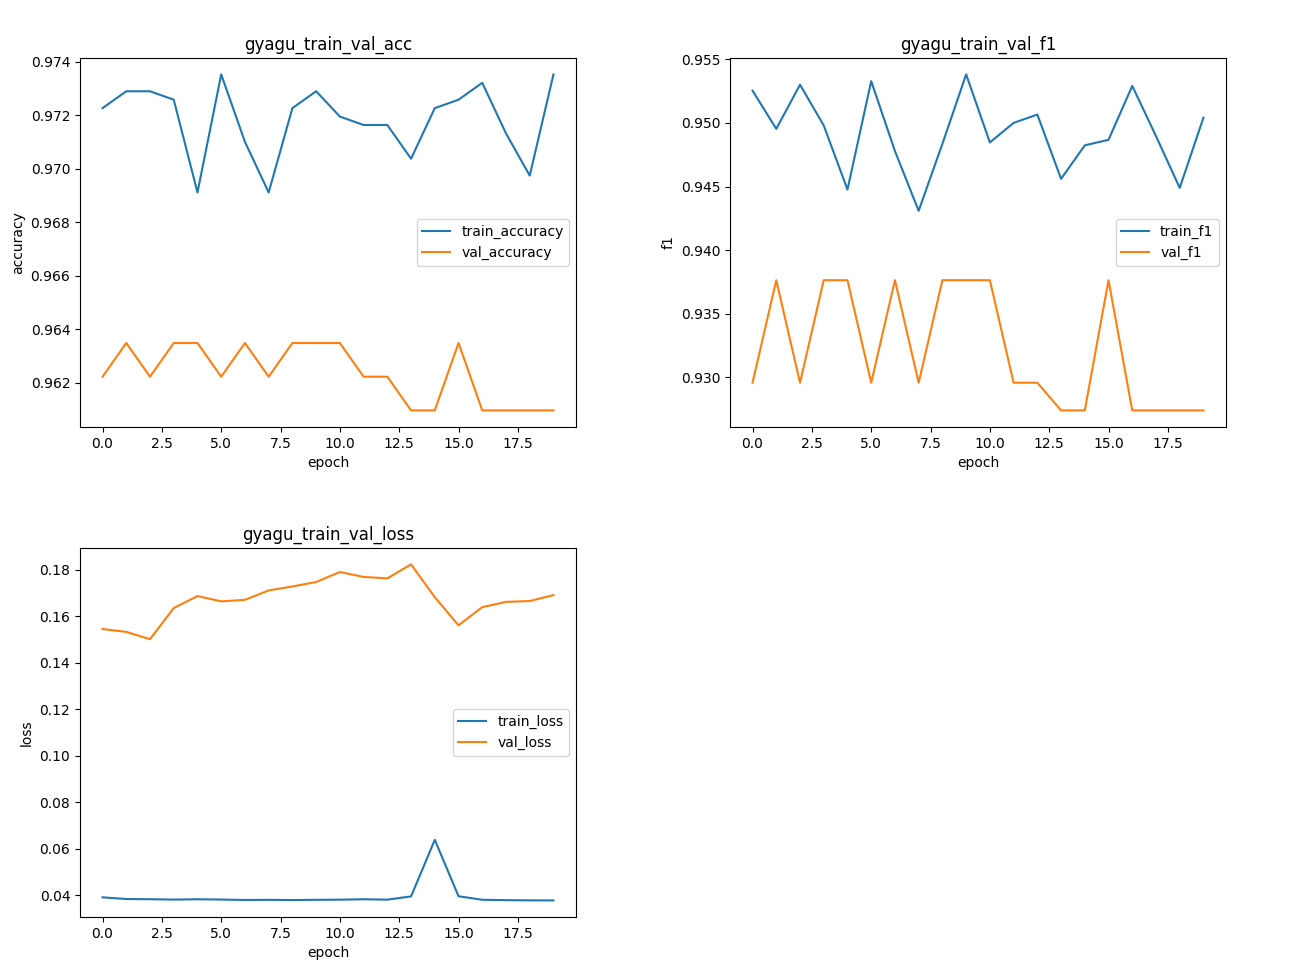
\includegraphics[width=8.0cm]{gyagu_res.png}
    \caption{gyagu graphs} %タイトルをつける
    \label{fig:gyagu} %ラベルをつけ図の参照を可能にする
  \end{center}
\end{figure}

\section{``1g-hub/bert\_practice" レポジトリ作成}

金田君と共に BERT の導入, 使い方の指南としてのレポジトリを作成した. 随時更新していく.
誤った情報などがあれば, 指摘をどうかよろしくお願いします.


\section{課題 優先度準}
\begin{itemize}
  \item BERT の fine-tuning 推敲. バグ探し.
  \item 他条件での BERT fine-tuning を行う.
  \item 新しく作成した d2v モデルと手法を用いた B3 実験の再実験および結果の比較.
  \item 森先生と大工大の上野先生に 30 話まであるらしい追加データをお願いする.
  \item Data Augmentation の手法の改善案.
\end{itemize}




\bibliographystyle{unsrt}
\bibliography{sankou}
\end{document}
